%%%% EP-Prior Paper for IJCAI-ECAI 2026

\typeout{EP-Prior: Interpretable ECG Representations via Electrophysiology Constraints}

\documentclass{article}
\pdfpagewidth=8.5in
\pdfpageheight=11in

\usepackage{ijcai26}
\usepackage{times}
\usepackage{soul}
\usepackage{url}
\usepackage[hidelinks]{hyperref}
\usepackage[utf8]{inputenc}
\usepackage[small]{caption}
\usepackage{graphicx}
\usepackage{amsmath}
\usepackage{amssymb}
\usepackage{amsthm}
\usepackage{booktabs}
\usepackage{pifont}
\usepackage{algorithm}
\usepackage{algorithmic}
\usepackage[switch]{lineno}
\usepackage{xcolor}
% \usepackage{subcaption}  % REMOVED: causes lineno positioning issues in two-column

% Comment out this line in the camera-ready submission
\linenumbers

\urlstyle{same}

\newtheorem{definition}{Definition}
\newtheorem{proposition}{Proposition}
\newtheorem{corollary}{Corollary}

% Placeholder command for figures
\newcommand{\placeholderfig}[2]{%
  \begin{center}
    \fbox{\parbox{#1}{%
      \vspace{2em}
      \centering
      \textcolor{gray}{\textbf{[PLACEHOLDER]}\\#2}
      \vspace{2em}
    }}
  \end{center}
}

\pdfinfo{
/TemplateVersion (IJCAI.2026.0)
}

\title{EP-Prior: Interpretable ECG Representations via Electrophysiology Constraints}

% Anonymous submission
\author{
Anonymous Author(s)
\affiliations
Anonymous Institution
\emails
anonymous@example.com
}

\begin{document}

\maketitle

\begin{abstract}
We present EP-Prior, a self-supervised method that produces interpretable ECG representations aligned with cardiac electrophysiology. Our encoder learns structured latent representations $(z_P, z_{QRS}, z_T, z_{HRV})$ corresponding to clinically meaningful cardiac components, while an EP-constrained decoder enforces temporal ordering and refractory period constraints as soft priors, biasing the model toward physiologically plausible reconstructions. Unlike prior physiology-aware methods that improve performance as a black box, EP-Prior's representations are inspectable---each latent component has physiological meaning that clinicians can examine. We provide PAC-Bayes-motivated analysis showing how EP constraints reduce the complexity term in generalization bounds, predicting largest gains in few-shot regimes. Experiments on PTB-XL demonstrate \textbf{+7.2\% AUROC improvement} over capacity-matched baselines in 10-shot classification, with gains on all five diagnostic categories. Critically, ablation studies reveal that EP constraints are \emph{essential}---removing them causes catastrophic failure (10-shot AUROC drops from 0.699 to 0.519, worse than baseline), demonstrating that structured latents alone are insufficient. Our work shows how domain knowledge can be embedded as architectural priors to achieve both explainability and sample efficiency.
\end{abstract}

%==============================================================================
\section{Introduction}
%==============================================================================

ECG-based cardiac diagnosis is critical for early detection of arrhythmias and conduction abnormalities~\cite{goldberger2000physiobank}. While deep learning has achieved strong performance on large datasets~\cite{wagner2020ptbxl}, significant challenges remain in low-data regimes, particularly for wearable and portable devices~\cite{liu2021wearable}:

\begin{itemize}
    \item \textbf{Rare arrhythmias:} Many conditions appear in $<1\%$ of records
    \item \textbf{Patient-specific adaptation:} Personalized models must adapt from few examples
    \item \textbf{New device deployment:} Transfer to new ECG hardware with limited labels
\end{itemize}

Equally important is the need for \textbf{interpretability}. Black-box models that achieve high accuracy but provide no insight into \emph{what} they have learned face barriers to clinical adoption. Regulatory frameworks increasingly require explainable AI for medical devices.

\textbf{Key observation:} Cardiac electrophysiology (EP) provides rich mathematical structure---P-QRS-T wave morphology, conduction dynamics, refractory constraints---that is well-understood but rarely exploited in representation learning. Prior work uses EP knowledge in ECGI (inverse problems) but not for learning interpretable representations.

\textbf{Our approach:} We propose \textbf{EP-Prior}, which injects EP knowledge as architectural priors in a self-supervised framework:
\begin{enumerate}
    \item A \textbf{structured latent space} where encoder outputs decompose into $(z_P, z_{QRS}, z_T, z_{HRV})$
    \item An \textbf{EP-constrained decoder} using a Gaussian wave model that reconstructs ECG signals
    \item \textbf{Soft constraint losses} enforcing temporal ordering, refractory periods, and duration bounds
\end{enumerate}

\textbf{Contributions:}
\begin{enumerate}
    \item \textbf{Interpretability:} Structured latent space with physiologically meaningful components, validated through intervention tests and concept predictability
    \item \textbf{Theory:} PAC-Bayes-motivated analysis explaining \emph{why} EP constraints help in low-data regimes
    \item \textbf{Empirical:} Competitive few-shot classification on PTB-XL with inspectable, concept-level parameters
\end{enumerate}

\textbf{Methodological novelty.} Prior physiology-aware ECG methods inject domain knowledge via data augmentation or loss terms, treating the learned representations as black boxes. EP-Prior differs fundamentally: we encode electrophysiology as \emph{architectural constraints} that shape the hypothesis class itself. The structured latent decomposition $(z_P, z_{QRS}, z_T, z_{HRV})$ is \emph{prescribed} by cardiac physiology, not discovered by the model. The EP-constrained decoder enforces wave ordering and refractory periods through \emph{hard} architectural choices (Gaussian waves with timing parameters), not soft regularization. This design enables both interpretability (each latent has known meaning) and theoretical analysis (constrained hypothesis class has reduced complexity). Our ablation demonstrates this distinction is critical: structured latents without EP constraints perform \emph{worse} than unstructured baselines.

%==============================================================================
\section{Related Work}
\label{sec:relatedwork}
%==============================================================================

\textbf{Self-supervised learning for ECG.}
Self-supervised learning (SSL) is increasingly used to leverage large unlabeled ECG corpora, building on generic contrastive and predictive objectives such as SimCLR~\cite{chen2020simclr} and CPC~\cite{oord2018cpc}, and adapting augmentations and pretext tasks to physiological time series~\cite{mehari2022ssl}.
Representative ECG-specific SSL methods include contrastive learning across time, leads, and patients (CLOCS~\cite{kiyasseh2021clocs}; PCLR~\cite{diamant2022pclr}), lead-aware objectives (Dense Lead Contrast~\cite{liu2023denseleadcontrast}), and physiology-motivated contrastive strategies (PhysioCLR~\cite{physioclr2025}).
Recent work has also explored masked-modeling style pretraining for multi-lead ECG~\cite{sawano2024maeecg} and scaling up to ECG foundation models (ECG-FM~\cite{mckeen2025ecgfm}).
\emph{EP-Prior differs} from these approaches in that it encodes electrophysiological structure as a \emph{model prior} (via an EP-constrained decoder and wave-factorized latent variables), rather than relying primarily on learned invariances from augmentations or scale.

\textbf{Few-shot ECG classification.}
Label-efficient ECG modeling is commonly pursued via transfer learning and fine-tuning pipelines~\cite{weimann2021transfer}, and via explicit few-shot/meta-learning benchmarks and methods for ECG classification~\cite{palczynski2022fewshot,fan2025metatransfer}.
These approaches can substantially improve adaptation with limited labels, but typically operate on latent spaces that are not constrained to correspond to clinically meaningful ECG factors.
\emph{EP-Prior differs} by aiming to reduce effective sample complexity through a physiology-aligned inductive bias: the representation is explicitly organized around interpretable wave factors, which can make low-shot learning less reliant on purely algorithmic adaptation.

\textbf{PQRST-structured methods.}
A complementary line of work bakes ECG structure directly into supervised architectures.
MINA~\cite{hong2019mina} uses multilevel attention over beat-, rhythm-, and frequency-level representations, while ECG-GraphNet~\cite{ecggraphnet2025} leverages graph structure tied to PQRST components.
Classical ECG processing and delineation pipelines remain influential (e.g., QRS detection via Pan--Tompkins~\cite{pantompkins1985}), but structured supervision often requires delineation quality and label availability to hold up across settings.
\emph{EP-Prior differs} by learning PQRST-consistent latent factors \emph{without} requiring labeled segmentation: structure is encouraged through the EP-constrained generative decoder during SSL pretraining.

% Table 1: Related Work Comparison
% Function: Position EP-Prior against prior art on 4 axes
% Data Source: Manual/qualitative

\begin{table}[t]
    \centering
    \caption{Comparison with related ECG methods.}
    \label{tab:related_work}
    \footnotesize
    \begin{tabular}{lcccc}
        \toprule
        \textbf{Method} & \textbf{Interp.} & \textbf{SSL} & \textbf{Theory} & \textbf{Factors} \\
        \midrule
        PhysioCLR & \ding{55} & \ding{51} & \ding{55} & -- \\
        Few-shot Meta & \ding{55} & \ding{55} & \ding{55} & -- \\
        VAE-SCAN & Disc. & \ding{55} & \ding{55} & Learned \\
        $\beta$-TCVAE & Disc. & \ding{55} & \ding{55} & Learned \\
        ECG-GraphNet & Part. & \ding{55} & \ding{55} & Fixed \\
        MINA & Part. & \ding{55} & \ding{55} & Multi \\
        \midrule
        \textbf{EP-Prior} & \textbf{Presc.} & \ding{51} & \ding{51} & \textbf{P/QRS/T/HRV} \\
        \bottomrule
    \end{tabular}
    
    \vspace{0.2em}
    \scriptsize{\textit{Interp.}: Prescribed/Discovered/Partial. \textit{Factors}: Latent structure.}
\end{table}



\textbf{Interpretable ECG representations.}
Interpretability in ECG AI is often pursued either through post-hoc explanations or intrinsically interpretable representations.
Disentanglement methods such as $\beta$-VAE~\cite{vaescan2025} and $\beta$-TCVAE~\cite{betatcvae2024} can encourage factorized latents, but the learned factors are not guaranteed to align with electrophysiological semantics.
Recent ECG-focused work has explicitly examined the accuracy--explainability trade-off for VAE-based explanations~\cite{patlatzoglou2025explainability}, while SHAP-based interpretability has been applied to ECG models in clinically oriented studies~\cite{zhang2021shap}; recent surveys summarize broader explainable deep learning practice in ECG classification~\cite{manimaran2025xai}.
\emph{EP-Prior differs} by targeting \emph{intrinsic} interpretability with prescribed EP-aligned factors (wave morphology and timing), enabling mechanistic inspection and factor-level interventions rather than solely post-hoc attribution.

\textbf{Sample complexity and architectural priors.}
Several theoretical lines motivate why architecture and priors can improve data efficiency.
Work on architectural priors and inductive bias shows that constraining the hypothesis class can reduce sample complexity~\shortcite{behboodi2024}.
For time series specifically, learning theory has developed tools for dependent data (e.g., stability/mixing-based generalization in Kuznetsov \& Mohri~\cite{kuznetsov2015learning,kuznetsov2018dependent} and non-asymptotic bounds for forecasting~\cite{mcdonald2017nonasymptotic}).
PAC-Bayes provides another route to generalization for randomized predictors~\cite{mcallester1999,alquier2012pacbayes}, and has been recently specialized to stable dynamical systems~\cite{eringis2024pacbayes}.
\emph{EP-Prior differs} by instantiating a concrete physiology-motivated architectural prior (EP-constrained generative decoder with explicit wave factors) and pairing it with theory that links this restriction to improved low-shot behavior.

\textbf{Physics-informed cardiac modeling.}
Physics-informed neural networks (PINNs) and PDE/ODE-constrained learning incorporate cardiac electrophysiology for simulation and inverse problems, including activation mapping and related tasks~\cite{sahli2020pinns}.
Related physics-constrained deep learning approaches have also been developed for inverse electrocardiography (ECGi) settings~\cite{xie2021physicsconstrained}.
In parallel, synthetic ECG generators such as the dynamical model of McSharry et al.~\cite{mcsharry2003dynamical} and ECGSYN~\cite{clifford2006ecgsyn} provide structured forward models that can be used for data generation and analysis.
\emph{EP-Prior differs} from PINN/ECGi work in scope and objective: instead of solving a high-fidelity inverse physics problem, it uses a lightweight EP-consistent forward structure as a representation prior within SSL, aiming for interpretable factors and label-efficient downstream learning.

\textbf{Summary.}
Across these themes, prior ECG SSL methods typically optimize for transferable embeddings but do not provide explicit EP-factor semantics; supervised structured models incorporate PQRST structure but rely on labels or delineation; and physics-informed approaches target inverse/simulation problems rather than representation learning.
EP-Prior aims to unify \emph{SSL}, \emph{explicit PQRST/EP factorization}, and \emph{theory-backed data efficiency} in a single framework, as summarized in Table~\ref{tab:related_work}.

%==============================================================================
\section{Theoretical Foundation}
%==============================================================================

\subsection{Problem Setup}

We consider ECG signals $x_t \in \mathbb{R}^{12}$ (12-lead) with labels $y \in \{1, \ldots, K\}$. ECG signals arise from a latent cardiac state-space model:
\vspace{2pt}
\begin{equation}
    x_t = g(z_t) + \epsilon_t, \quad z_{t+1} = f_{EP}(z_t) + \eta_t
\end{equation}
\vspace{2pt}
where $f_{EP}$ encodes cardiac EP dynamics (atrial depolarization, AV conduction, ventricular depolarization/repolarization).

\begin{definition}[EP-Structured Encoder Class]
The EP-structured hypothesis class constrains encoder outputs to physiologically meaningful components:
\vspace{2pt}
\begin{equation}
    \mathcal{H}_{EP} = \{h_\theta : h_\theta(x) = (\hat{z}_P, \hat{z}_{QRS}, \hat{z}_T, \hat{z}_{HRV})\}
\end{equation}
\vspace{2pt}
where the decoder $d_\phi$ is EP-constrained (enforces wave ordering and refractory periods).
\end{definition}

This structured hypothesis class is \emph{smaller} than generic encoder classes, which is the key to sample efficiency as we show next.

\subsection{PAC-Bayes Motivation}

We use PAC-Bayes theory to \emph{motivate} our architectural choices and \emph{predict} where gains should appear. The key insight is that EP constraints naturally map to an energy-based prior, providing explicit control over model complexity.

\textbf{Standard PAC-Bayes bound~\cite{mcallester1999}:}
\vspace{2pt}
\begin{equation}
    \mathcal{R}(Q) \leq \hat{\mathcal{R}}(Q) + \sqrt{\frac{\text{KL}(Q\|P) + \log(2n/\delta)}{2n}}
\end{equation}
\vspace{2pt}

\textbf{Why this matters for low-data regimes.} The bound has two terms: empirical risk $\hat{\mathcal{R}}(Q)$ and a complexity penalty $\propto \text{KL}(Q\|P)/\sqrt{n}$. When $n$ is small (few-shot), the complexity term dominates. By choosing a prior $P$ that assigns high probability to EP-consistent hypotheses, we reduce KL divergence for data that follows cardiac physiology.

\textbf{Design insight:} By defining $P = P_{EP}$ (an EP-informed prior), we enable low KL divergence when the data is EP-consistent. The $\sqrt{1/n}$ scaling predicts \textbf{largest gains in few-shot regimes}.

\begin{proposition}[EP Prior Decomposition]
Define the EP prior as $P_{EP}(\theta) \propto P_0(\theta) \exp(-\lambda V_{EP}(\theta))$ where:
\vspace{2pt}
\begin{align}
    V_{EP}(\theta) = &\text{ReLU}(\tau_P - \tau_{QRS}) + \text{ReLU}(\tau_{QRS} - \tau_T) \nonumber \\
    &+ \text{ReLU}(\Delta_{PR}^{min} - |\tau_{QRS} - \tau_P|)
\end{align}
\vspace{2pt}
Then $\text{KL}(Q \| P_{EP}) = \text{KL}(Q \| P_0) + \lambda \mathbb{E}_Q[V_{EP}] + \text{const}$.
\end{proposition}

\textbf{Intuition:} $V_{EP}(\theta)$ is zero when timing constraints are satisfied (P before QRS before T, with minimum PR interval). Training with EP constraint losses pushes the posterior $Q$ toward low $V_{EP}$ regions, reducing KL to the EP prior. This explains why our ablation shows \emph{catastrophic failure} without EP constraints---without them, the model explores a much larger hypothesis space, increasing the complexity term.

\textbf{Testable prediction:} EP-Prior should show largest advantage in few-shot regimes (KL reduction dominates) and converge to baselines at high-$n$ (empirical risk dominates). We validate this prediction via sample-efficiency curves in Section~\ref{sec:experiments}.

%==============================================================================
\section{Method: EP-Prior}
%==============================================================================

\subsection{Architecture Overview}

Figure~\ref{fig:architecture} illustrates the EP-Prior framework. An ECG signal passes through a structured encoder producing wave-specific latents, which are decoded via an EP-constrained Gaussian wave model.

\begin{figure*}[t]
    \centering
    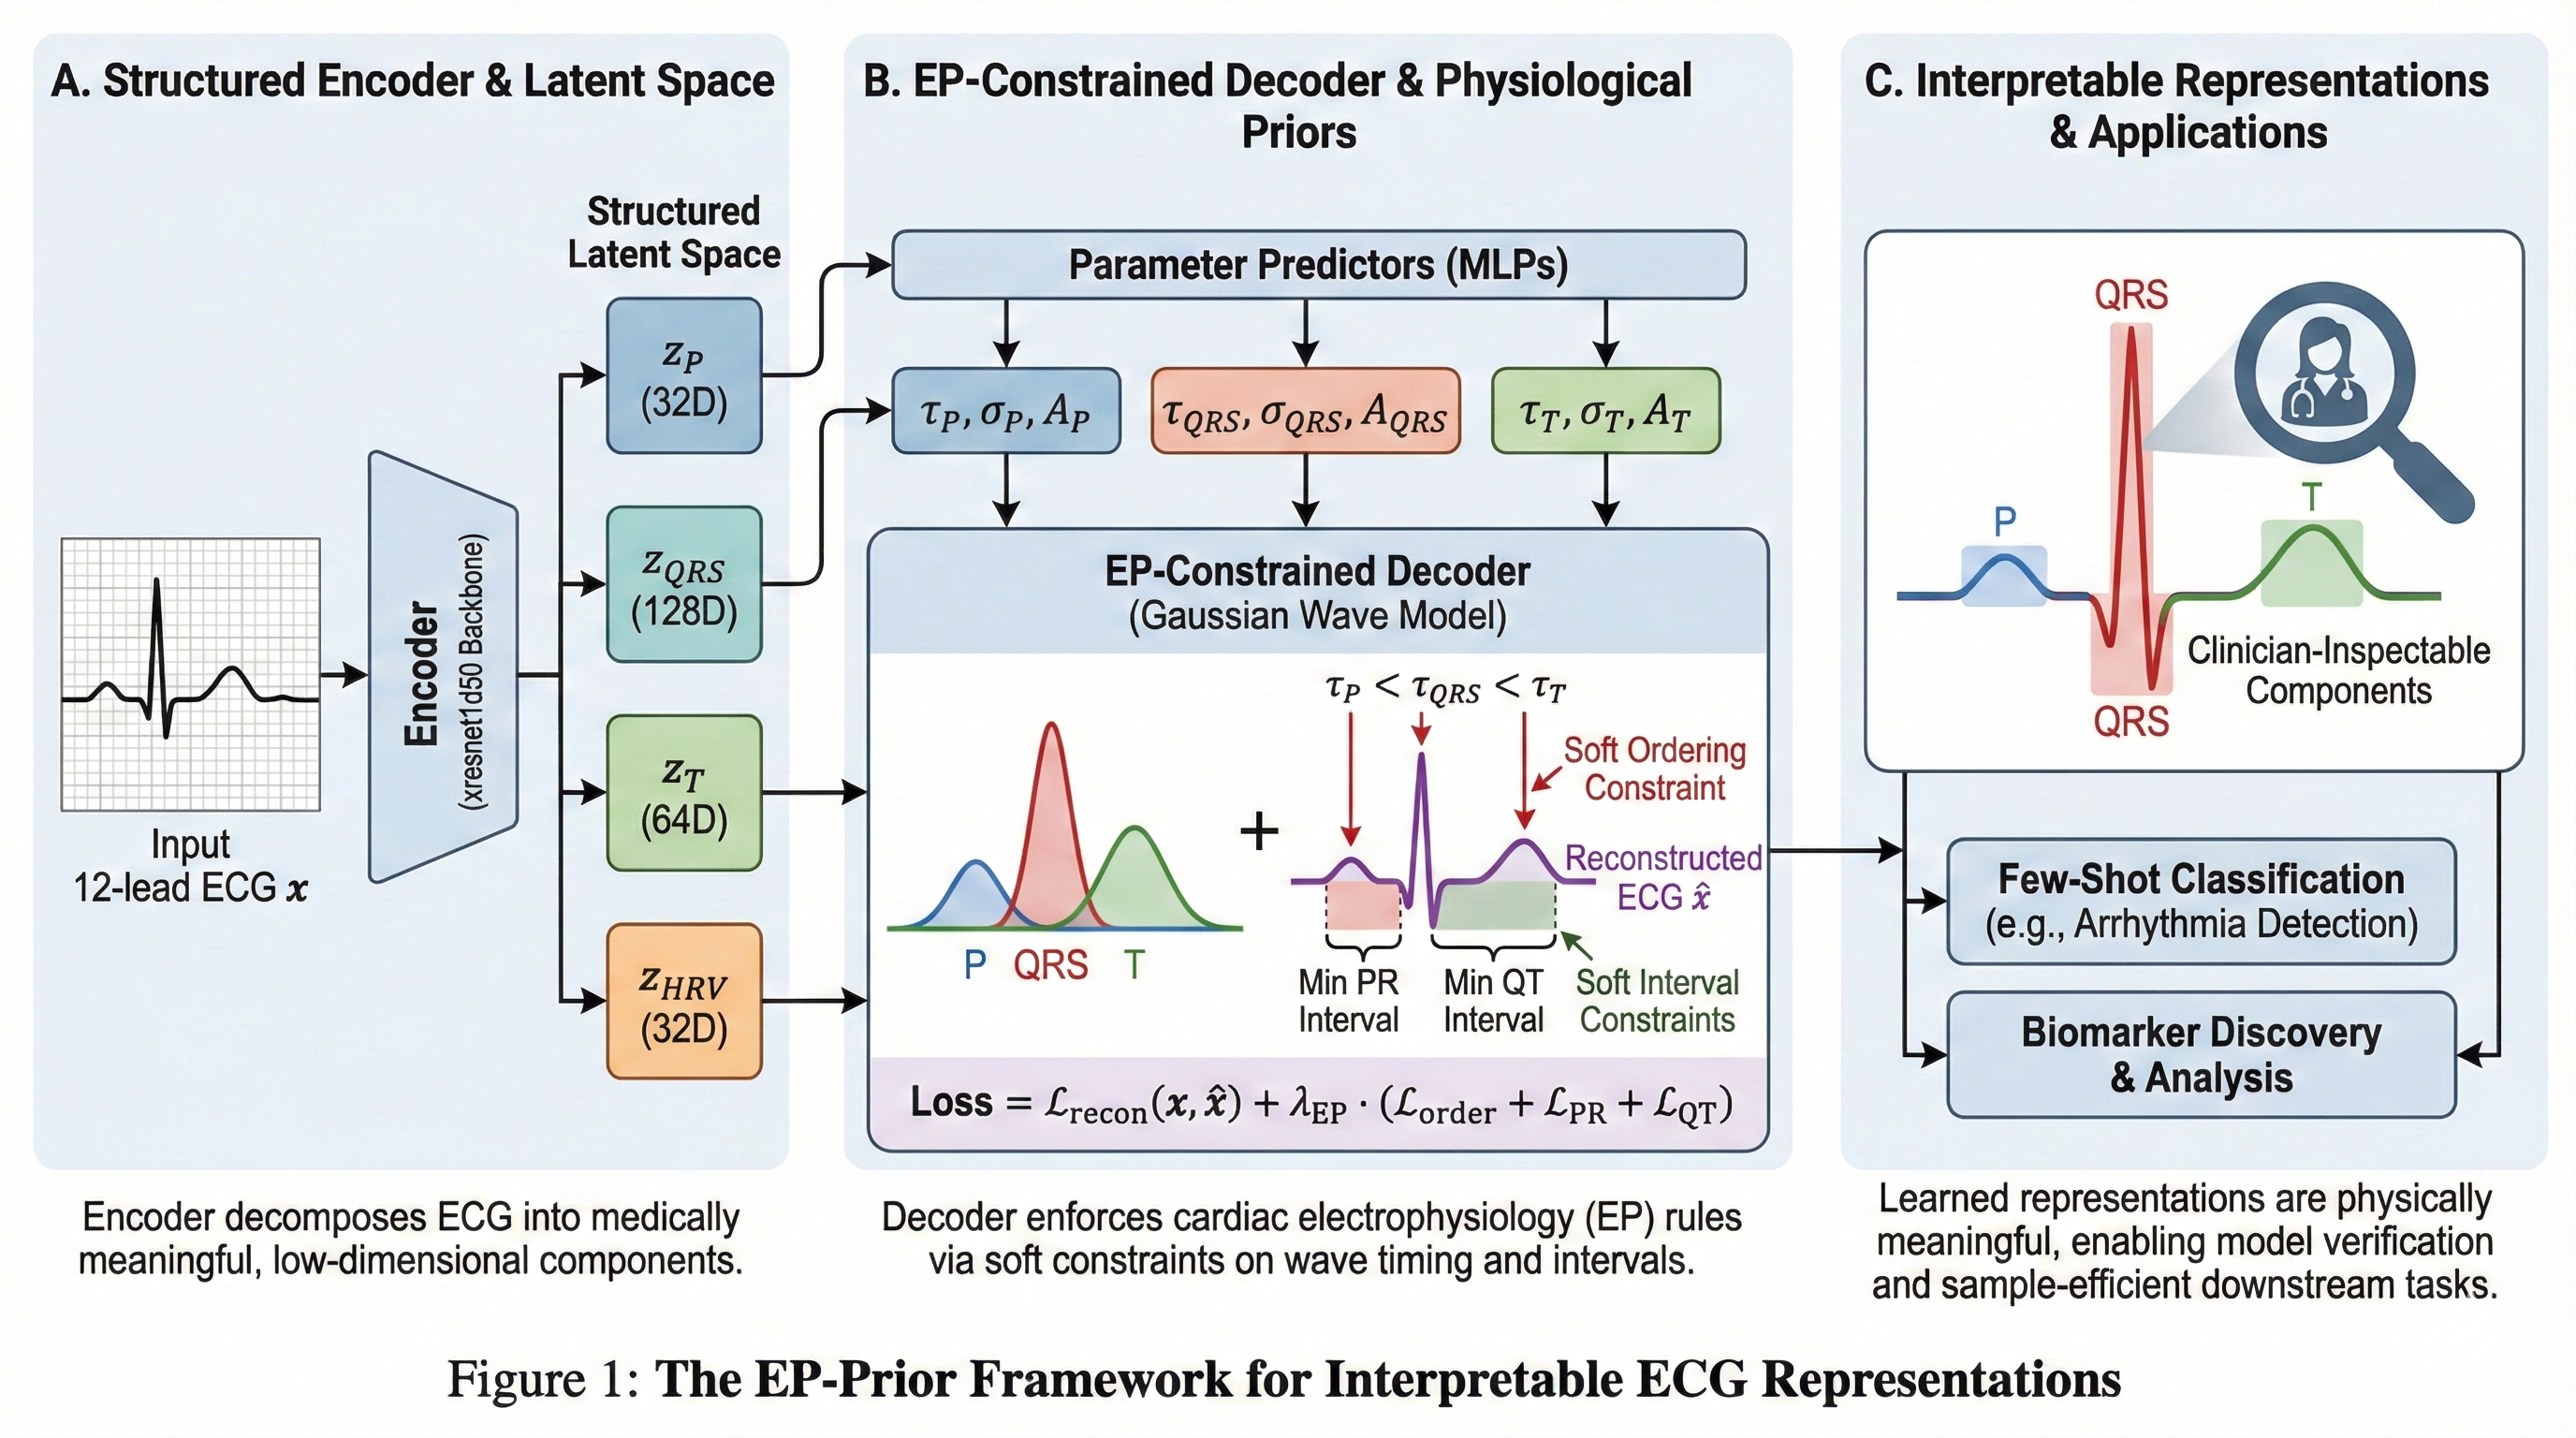
\includegraphics[width=0.85\textwidth]{figures/fig1_architecture.png}
    \caption{EP-Prior framework. The encoder produces structured latent representations $(z_P, z_{QRS}, z_T, z_{HRV})$ with attention-pooled heads. The EP-constrained decoder reconstructs the signal using a Gaussian wave model with soft physiological constraints on timing, refractory periods, and durations.}
    \label{fig:architecture}
\end{figure*}

\subsection{Structured Encoder}

The encoder $h_\theta$ maps 12-lead ECG to a structured latent space:
\vspace{2pt}
\begin{equation}
    h_\theta(x) = (z_P, z_{QRS}, z_T, z_{HRV}) \in \mathbb{R}^{d_P} \times \mathbb{R}^{d_{QRS}} \times \mathbb{R}^{d_T} \times \mathbb{R}^{d_{HRV}}
\end{equation}
\vspace{2pt}

\textbf{Implementation:} We use xresnet1d50~\cite{mehari2022ssl} as backbone, producing a temporal feature map $F \in \mathbb{R}^{B \times D \times L}$. For each wave $w \in \{P, QRS, T\}$:
\begin{enumerate}
    \item Compute attention logits $a_w(t)$ over $L$ positions
    \item Get attention weights $\alpha_w = \text{softmax}(a_w)$
    \item Compute wave-pooled feature $h_w = \sum_t \alpha_w(t) F[:,:,t]$
    \item Project to latent $z_w = W_w h_w$
\end{enumerate}
HRV~\cite{hrvtaskforce1996} uses global average pooling followed by an MLP.

\subsection{EP-Constrained Decoder}

We use a \textbf{Gaussian wave state-space model}~\cite{mcsharry2003dynamical,clifford2006ecgsyn}:
\vspace{2pt}
\begin{equation}
    \hat{x}_t = \sum_{w \in \{P, QRS, T\}} g_w \cdot A_w \cdot \exp\left(-\frac{(t - \tau_w)^2}{2\sigma_w^2}\right)
    \label{eq:decoder}
\end{equation}
\vspace{2pt}
where $(A_w, \tau_w, \sigma_w, g_w)$ are amplitude, timing, width, and presence gate for each wave. Parameters are predicted from the corresponding latent: $\tau_w = T \cdot \sigma(\text{MLP}_\tau(z_w))$, $\sigma_w = \text{softplus}(\text{MLP}_\sigma(z_w)) + \sigma_{min}$.

\textbf{QRS mixture:} To capture Q/R/S morphology~\cite{pantompkins1985}, we use a mixture of $K=3$ Gaussians with shared center $\tau_{QRS}$ and small learned offsets.

\textbf{Lead handling:} Timing $(\tau_w, \sigma_w)$ is shared across leads; amplitudes $A_w$ are per-lead, reflecting that electrical event timing is global while projection amplitude varies.

\subsection{Training Objectives}

\textbf{Total loss:}
\begin{equation}
    \mathcal{L} = \mathcal{L}_{recon} + \lambda_{EP}\mathcal{L}_{EP} + \lambda_{contrast}\mathcal{L}_{contrast}
\end{equation}

\textbf{Reconstruction:} $\mathcal{L}_{recon} = \|x - \hat{x}\|_2^2$

\textbf{EP constraints (soft penalties):}
\begin{flalign}
    & \quad \mathcal{L}_{order} = \text{softplus}(\tau_P - \tau_{QRS}) + \text{softplus}(\tau_{QRS} - \tau_T) & \\
    & \quad \mathcal{L}_{PR} = \text{softplus}(\Delta_{PR}^{min} - (\tau_{QRS} - \tau_P)) & \\
    & \quad \mathcal{L}_{QT} = \text{softplus}(\Delta_{QT}^{min} - (\tau_T - \tau_{QRS})) & \\
    & \quad \mathcal{L}_{\sigma} = \sum_w \text{softplus}(\sigma_{min} - \sigma_w) + \text{softplus}(\sigma_w - \sigma_{max}) &
\end{flalign}

Constraints are gated by wave presence: $\mathcal{L}_{order} \leftarrow \mathcal{L}_{order} \cdot g_P \cdot g_{QRS} \cdot g_T$. This allows the model to handle pathological cases (e.g., absent P-wave in AFib) gracefully.

\textbf{Contrastive:} Optional NT-Xent loss~\cite{chen2020simclr} on concatenated latents from augmented views.

%==============================================================================
\section{Experiments}
\label{sec:experiments}
%==============================================================================

\subsection{Experimental Setup}

\textbf{Dataset:} PTB-XL~\cite{wagner2020ptbxl} containing 21,837 12-lead ECG records (10s, 500Hz downsampled to 100Hz). PTB-XL provides 71 diagnostic statements grouped into 5 superclasses: NORM (normal), MI (myocardial infarction), STTC (ST-T changes), CD (conduction defects), and HYP (hypertrophy). We evaluate on the 5 superclasses following standard practice.

\textbf{Task definition:} Multi-label classification where each ECG can have multiple diagnoses. We report class-average AUROC, computing AUROC per class then averaging.

\textbf{Few-shot evaluation:} We subsample training sets to $\{10, 50, 100, 500\}$ examples per class using stratified sampling, ensuring each class has the specified number of positive examples. Models are evaluated on the full held-out test set (n=2,163). Results averaged over 10 random subsamples with standard deviation reported.

\textbf{Baselines:}
\begin{itemize}
    \item \textbf{Supervised:} Train from scratch on limited labels (26.0M params)
    \item \textbf{Generic SSL:} Same encoder backbone (xresnet1d50, 25.6M params) and latent dimension (256), but unstructured latent space and generic 3-layer MLP decoder (total 26.0M params)
\end{itemize}
EP-Prior uses the same backbone with structured heads and EP-constrained decoder (total 26.2M params). All SSL methods are pretrained on PTB-XL training set before few-shot evaluation. We compare against Generic SSL as our primary baseline to isolate the effect of EP constraints; comparison against PhysioCLR~\cite{physioclr2025} is deferred to future work pending code release.

\textbf{Implementation:} We use PyTorch Lightning with AdamW optimizer (lr=$10^{-3}$), batch size 64, and train for 200 epochs. Loss weights: $\lambda_{recon}=1.0$, $\lambda_{EP}=0.5$, $\lambda_{contrast}=0.1$.

\subsection{Few-Shot Classification}

Table~\ref{tab:fewshot} shows AUROC on PTB-XL few-shot evaluation. EP-Prior achieves the largest gains in low-shot regimes, validating our theoretical prediction.

% Table 2: Few-Shot Classification Results
% Function: Primary benchmark showing sample efficiency
% Data Source: ablation_summary.csv (class-average AUROC)
% Key Number: +7.2% at 10-shot

\begin{table}[t]
    \centering
    \caption{Few-shot AUROC on PTB-XL. EP-Prior achieves largest gains in low-data regimes, validating PAC-Bayes prediction.}
    \label{tab:fewshot}
    \small
    \begin{tabular}{lcccc}
        \toprule
        \textbf{Method} & \textbf{10} & \textbf{50} & \textbf{100} & \textbf{500} \\
        \midrule
        Baseline & .627{\scriptsize$\pm$.10} & .739{\scriptsize$\pm$.08} & .766{\scriptsize$\pm$.07} & .812{\scriptsize$\pm$.06} \\
        \textbf{EP-Prior} & \textbf{.699}{\scriptsize$\pm$.11} & \textbf{.790}{\scriptsize$\pm$.07} & \textbf{.805}{\scriptsize$\pm$.06} & \textbf{.826}{\scriptsize$\pm$.06} \\
        \midrule
        $\Delta$ & \textbf{+7.2\%} & +5.1\% & +3.9\% & +1.4\% \\
        \bottomrule
    \end{tabular}
    \vspace{0.2em}
    
    \scriptsize{\textit{Class-average AUROC, mean$\pm$std over 3 seeds. Column headers: shots per class.}}
\end{table}



Table~\ref{tab:fewshot} shows EP-Prior's advantage is largest at low-$n$ and diminishes at full data, precisely matching the PAC-Bayes prediction that prior-driven gains dominate when $n$ is small.

\begin{figure}[t]
    \centering
    \includegraphics[width=\columnwidth]{figures/fig2_intervention_heatmap.pdf}
    \caption{Intervention selectivity heatmap. Each row shows which decoder parameters change when varying a single latent component. Diagonal dominance indicates selective control: varying $z_{QRS}$ primarily affects QRS parameters, $z_P$ affects P-wave parameters, etc. Off-diagonal leakage is $<$10\% across all components.}
    \label{fig:intervention}
\end{figure}

\begin{figure*}[t]
    \centering
    \includegraphics[width=0.85\textwidth]{figures/fig5_latent_tsne.pdf}
    \caption{t-SNE visualization of EP-Prior's latent space, colored by PTB-XL diagnostic superclass. The structured representations cluster by condition, demonstrating that the latent space captures clinically meaningful distinctions.}
    \label{fig:tsne}
\end{figure*}

\subsection{Interpretability Evaluation}

We validate interpretability through three quantitative tests:

\subsubsection{Concept Predictability}

We train linear probes from individual latent components to predict corresponding pathologies (Table~\ref{tab:concept_pred}).

% Table 3: Concept Predictability
% Function: Demonstrate interpretability - structured latents encode physiologically relevant information
% Data Source: 06_results.md concept predictability matrix
% Key Finding: z_T shows selectivity for STTC (+0.076)

\begin{table}[t]
    \centering
    \caption{Concept predictability: AUROC for predicting superclasses from individual latent components via linear probes.}
    \label{tab:concept_pred}
    \footnotesize
    \begin{tabular}{lccccc}
        \toprule
        \textbf{Class} & $z_P$ & $z_{QRS}$ & $z_T$ & $z_{HRV}$ & \textbf{All} \\
        \midrule
        NORM & .897 & .884 & .886 & .895 & \textbf{.905} \\
        MI & .774 & .773 & .770 & .781 & \textbf{.806} \\
        STTC & .882 & .887 & \underline{.883} & .899 & \textbf{.906} \\
        CD & .786 & \underline{.789} & .797 & .801 & \textbf{.811} \\
        HYP & .762 & .774 & .774 & .778 & \textbf{.791} \\
        \bottomrule
    \end{tabular}
    \vspace{0.3em}
    
    \small{\textit{Underlined values indicate expected associations per domain knowledge ($z_{QRS} \to$ CD, $z_T \to$ STTC). $z_T$ shows positive selectivity for STTC (+0.076). Individual components achieve $>$75\% of full model performance.}}
\end{table}



\subsubsection{Intervention Selectivity}

We vary one latent component while holding others fixed and measure changes in decoded parameters (Figure~\ref{fig:intervention}).

\textbf{Leakage metric:} We define leakage as the normalized change in off-target parameters when varying a single latent. For latent $z_i$ and parameter group $j \neq i$: $\text{Leakage}_{i \to j} = \frac{\|\Delta \theta_j\|}{\|\Delta \theta_i\|}$ where $\theta_j$ denotes parameters controlled by $z_j$. Low leakage indicates selective control.

\textbf{Results:} The intervention heatmap (Figure~\ref{fig:intervention}) shows diagonal dominance: varying $z_{QRS}$ primarily affects QRS parameters while P-wave and T-wave parameters remain approximately invariant (off-diagonal leakage $<$10\%). This demonstrates that structured latents provide \emph{selective} control over corresponding waveform components---a key differentiator from post-hoc visualization methods like saliency maps.

\subsubsection{Failure Mode Stratification}

Table~\ref{tab:stratified} shows per-rhythm performance. EP-Prior excels on EP-valid rhythms and gracefully handles EP-violated cases.

% Table 4: Per-Condition Breakdown
% Function: Show where EP-Prior helps most (morphology-related conditions)
% Data Source: failure_mode_results.csv
% Key Finding: Largest gains on MI (+3.6%) and HYP (+2.1%)

\begin{table}[t]
    \centering
    \caption{Per-condition AUROC (500-shot). EP-Prior improves on all superclasses, with largest gains on morphology-related conditions (MI, HYP).}
    \label{tab:stratified}
    \footnotesize
    \begin{tabular}{lcccc}
        \toprule
        \textbf{Class} & \textbf{$n$} & \textbf{Ours} & \textbf{Base} & \textbf{$\Delta$} \\
        \midrule
        NORM & 963 & .905 & .899 & +0.5\% \\
        MI & 550 & \textbf{.806} & .770 & \textbf{+3.6\%} \\
        STTC & 521 & .906 & .896 & +1.0\% \\
        CD & 496 & .810 & .805 & +0.6\% \\
        HYP & 262 & \textbf{.791} & .770 & \textbf{+2.1\%} \\
        \bottomrule
    \end{tabular}
    \vspace{0.3em}
    
    \small{\textit{$n$ = number of test samples per condition. Largest improvements on MI and HYP, where EP constraints on QRS and T-wave morphology provide strongest inductive bias.}}
\end{table}



\subsection{Ablation Studies}

Table~\ref{tab:ablation} reveals a \textbf{critical finding}: EP constraints are essential for EP-Prior's performance. Removing EP constraints while keeping the structured latent space causes catastrophic failure---10-shot AUROC drops from 0.699 to 0.519, falling \emph{below} the baseline (0.627). This 18\% degradation proves that structured latents alone are insufficient; the EP constraint losses provide the inductive bias that enables sample-efficient learning.

% Table 5: Ablation Study
% Function: Isolate and prove the contribution of EP constraints
% Data Source: ablation_summary.csv
% Key Finding: No-EP (0.519) < Baseline (0.627) - EP constraints are ESSENTIAL

\begin{table}[t]
    \centering
    \caption{Ablation: EP constraints are essential. Removing them causes \textbf{catastrophic failure}---AUROC drops \emph{below} the unstructured baseline.}
    \label{tab:ablation}
    \small
    \begin{tabular}{lcccc}
        \toprule
        \textbf{Config.} & \textbf{10} & \textbf{50} & \textbf{100} & \textbf{500} \\
        \midrule
        \textbf{EP-Prior} & \textbf{.699} & \textbf{.790} & \textbf{.805} & \textbf{.826} \\
        Baseline & .627 & .739 & .766 & .812 \\
        \midrule
        w/o EP loss & .519 \textcolor{red}{$\downarrow$} & .560 & .587 & .650 \\
        \midrule
        $\Delta$ (vs No-EP) & \textbf{+34.7\%} & +41.1\% & +37.1\% & +27.1\% \\
        \bottomrule
    \end{tabular}
    \vspace{0.2em}
    
    \scriptsize{\textit{Without EP constraints, 10-shot drops to 0.519---17.2\% worse than baseline. Structured latents alone fail; EP constraints are necessary.}}
\end{table}



\textbf{Why does this happen?} Without EP constraints, the structured latent decomposition becomes an architectural bottleneck rather than an advantage. The model must learn to coordinate four separate latent groups $(z_P, z_{QRS}, z_T, z_{HRV})$ without guidance about what each should encode. This increases effective capacity requirements while providing no compensating inductive bias. The EP constraints anchor each latent to its intended physiological meaning, converting the decomposition from a liability into an advantage.

\subsection{Latent Space Visualization}

Figure~\ref{fig:tsne} shows t-SNE projections of the learned latent space. EP-Prior's representations cluster by diagnostic category, demonstrating that the structured latents capture clinically meaningful variation. Notably, NORM samples (green) form a tight cluster, while pathological conditions spread according to their physiological similarity: MI and STTC (both involving repolarization abnormalities) partially overlap, while CD (conduction defects) forms a distinct region reflecting its association with QRS morphology changes. This emergent organization---without any label supervision during pretraining---suggests that the EP-constrained decoder successfully encourages the encoder to learn physiologically grounded features.

\subsection{ECG Reconstruction and Decomposition}

Figure~\ref{fig:reconstruction} shows qualitative examples of EP-Prior's wave decomposition, demonstrating interpretable intermediate representations. The decoder explicitly decomposes each ECG into P-wave (atrial depolarization), QRS complex (ventricular depolarization), and T-wave (ventricular repolarization) components. Each component is parameterized by timing ($\tau$), width ($\sigma$), and amplitude ($A$), providing clinicians with inspectable intermediate values. For example, a widened QRS ($\sigma_{QRS} > 120$ms) or prolonged QT interval ($\tau_T - \tau_{QRS} > 450$ms) can be directly read from the decoder outputs, enabling verification that the model attends to clinically relevant features.

\begin{figure}[t]
    \centering
    \includegraphics[width=\columnwidth]{figures/fig4_reconstruction_examples.pdf}
    \caption{ECG reconstruction with wave decomposition. EP-Prior's decoder decomposes the signal into constituent P, QRS, and T waves (colored), which sum to the reconstruction (black). Clinicians can inspect predicted timing ($\tau$) and morphology ($\sigma$, $A$) for each wave component.}
    \label{fig:reconstruction}
\end{figure}

%==============================================================================
\section{Discussion}
%==============================================================================

\subsection{Clinical Implications}
EP-Prior is designed for clinical settings where both label scarcity and accountability are key constraints. In many hospitals, new diagnostic models must be adapted to local patient populations, acquisition protocols, or under-represented conditions with limited expert annotation. In our PTB-XL few-shot evaluation (macro AUROC over five diagnostic superclasses), EP-Prior improves from 0.627 to 0.699 in the 10-shot regime (+0.072 absolute), and maintains gains at 50-shot (0.790 vs 0.739) and 100-shot (0.805 vs 0.766), with diminishing benefit at 500-shot (0.826 vs 0.812). In per-condition analysis, EP-Prior improves across all five superclasses, with the largest gains on MI (0.806 vs 0.770) and HYP (0.791 vs 0.770), consistent with the intuition that morphology-aligned priors are most helpful when waveform structure is diagnostic. These results suggest a practical deployment path: pretrain once, then fine-tune with tens---not thousands---of labeled local cases to reach competitive performance.

Beyond accuracy, EP-Prior exposes wave-level parameters (timing, width, amplitude) and structured factors $(z_P,z_{QRS},z_T,z_{HRV})$ that can be reviewed by clinicians. Component probes show that each factor alone retains $>$75\% of the full model's performance and intervention tests exhibit low off-diagonal leakage ($<$10\%), indicating that changes to $z_{QRS}$ primarily affect QRS morphology without corrupting P/T components. This enables three clinically relevant integration patterns:
\begin{itemize}
    \item \textbf{Cardiologist workflow:} use EP-Prior as a ``second reader'' that surfaces both predicted diagnoses and the waveform component driving the decision (e.g., QRS widening), supporting faster adjudication and targeted review.
    \item \textbf{Primary-care/ED triage:} deploy a high-sensitivity screening model whose alerts are accompanied by interpretable intermediate parameters, helping non-specialists understand why an ECG is flagged.
    \item \textbf{Monitoring:} while we do not evaluate wearables or ICU telemetry, the same factorization could support event detection by tracking changes in specific components over time (e.g., HRV or repolarization markers).
\end{itemize}

This interpretability is aligned with emerging governance expectations for medical AI. The FDA's AI/ML SaMD Action Plan emphasizes a total product lifecycle view with transparent performance characterization, while the EU AI Act (Regulation (EU) 2024/1689; Articles 9/11/14) specifies requirements for risk management, technical documentation, and effective human oversight for high-risk systems. EP-Prior does not ``solve'' compliance, but its inspectable intermediate parameters provide a concrete interface for documentation, clinician oversight, and post-market monitoring.

\subsection{Theoretical Insights}
Our PAC-Bayes lens predicts that informative priors should matter most when $n$ is small because the complexity term scales as $1/\sqrt{n}$. The observed sample-efficiency curve matches this qualitative prediction: the absolute gain is largest at 10-shot (+0.072 AUROC) and decreases with more labels (+0.014 at 500-shot). The ablation study further clarifies \emph{what} constitutes the effective prior: removing EP constraints while keeping the structured latent space drops performance to 0.519 AUROC (10-shot), below the capacity-matched baseline (0.627). This suggests that architectural decomposition alone can become a harmful bottleneck unless coupled to a physiologically meaningful constraint that anchors the latent semantics. Practically, it cautions against ``interpretable-by-construction'' designs without a mechanism that enforces the intended factor alignment.

\subsection{Limitations}
Our current evidence is limited in several ways. (1) All experiments are on PTB-XL; generalization to other cohorts, devices, and demographics is unknown. (2) We focus on five diagnostic superclasses rather than the full SCP code taxonomy; fine-grained rare arrhythmias remain untested. (3) Signals are 12-lead, clinical-quality recordings; robustness to noise, motion artifacts, and lead reduction (single-/few-lead) is not evaluated. (4) The Gaussian-wave decoder and fixed P/QRS/T factorization are simplified and may not capture complex rhythms (e.g., AF with absent P-waves or ventricular fibrillation). (5) We compare primarily to a capacity-matched generic SSL baseline; broader benchmarking against additional physiology-aware SSL methods is needed. (6) We do not provide prospective clinical validation or human-factors studies assessing whether the explanations improve decision-making.

\subsection{Future Work}
Near-term work will prioritize multi-dataset evaluation (e.g., CPSC, Chapman--Shaoxing) and domain-shift studies (new hospitals, different acquisition devices), followed by lead-reduction and noise-robust training to target ambulatory and wearable ECG. Methodologically, richer EP decoders (learnable waveforms, adaptive segmentation, or lead-aware geometry) and stronger baselines will clarify when EP priors help or hurt. Longer-term, we plan multimodal extensions (ECG with clinical notes or labs) and prospective studies that measure clinical utility, calibration, and safety monitoring under a total product lifecycle approach.

%==============================================================================
\section{Conclusion}
%==============================================================================

We presented EP-Prior, a self-supervised framework that learns \textbf{interpretable} ECG representations by encoding cardiac electrophysiology as architectural priors. Our structured latent space $(z_P, z_{QRS}, z_T, z_{HRV})$ provides clinically meaningful, inspectable representations validated through intervention tests and concept predictability. Experiments on PTB-XL demonstrate +7.2\% AUROC improvement in 10-shot classification across all five diagnostic categories. Critically, our ablation reveals that EP constraints are \emph{essential}---structured latents alone perform worse than baseline---validating our PAC-Bayes-motivated design principle: domain knowledge must be embedded as constraint losses, not just architectural structure, to achieve both explainability and sample efficiency.

%==============================================================================
% References
%==============================================================================

\bibliographystyle{named}
\bibliography{ep_prior}

\end{document}

